\documentclass[margin=5mm]{standalone}
\usepackage{tikz}
\usetikzlibrary{positioning, fit, calc, arrows.meta, shapes.geometric}
\usepackage{helvet}
\renewcommand{\familydefault}{\sfdefault}

% ==========================================
% Definición de la paleta de colores
% ==========================================
\definecolor{boxblue}{RGB}{165,216,255}
\definecolor{borderblue}{RGB}{25,113,194}
\definecolor{boxgreen}{RGB}{209,250,229}
\definecolor{bordergreen}{RGB}{5,150,105}
\definecolor{boxorange}{RGB}{254,215,170}
\definecolor{borderorange}{RGB}{234,88,12}
\definecolor{boxgray}{RGB}{226,232,240}
\definecolor{bordergray}{RGB}{100,116,139}
\definecolor{textred}{RGB}{220,38,38}

% ==========================================
% Estilos globales de nodos y flechas
% ==========================================
\tikzset{
    basebox/.style={
        align=center,
        rounded corners=4pt,
        thick,
        font=\small,
        inner sep=6pt
    },
    bluebox/.style={basebox, fill=boxblue, draw=borderblue, minimum width=3.8cm, minimum height=1cm},
    greenbox/.style={basebox, fill=boxgreen, draw=bordergreen, minimum width=3.8cm, minimum height=1cm},
    widegreenbox/.style={basebox, fill=boxgreen, draw=bordergreen, minimum width=12cm, minimum height=1cm},
    graybox/.style={basebox, fill=boxgray, draw=bordergray, minimum width=5.5cm, minimum height=1cm},
    myarrow/.style={-{Stealth[length=3mm]}, thick, draw=black!80},
    mydashedarrow/.style={-{Stealth[length=3mm]}, thick, dashed, draw=black!80}
}

\begin{document}
\pagecolor{white}
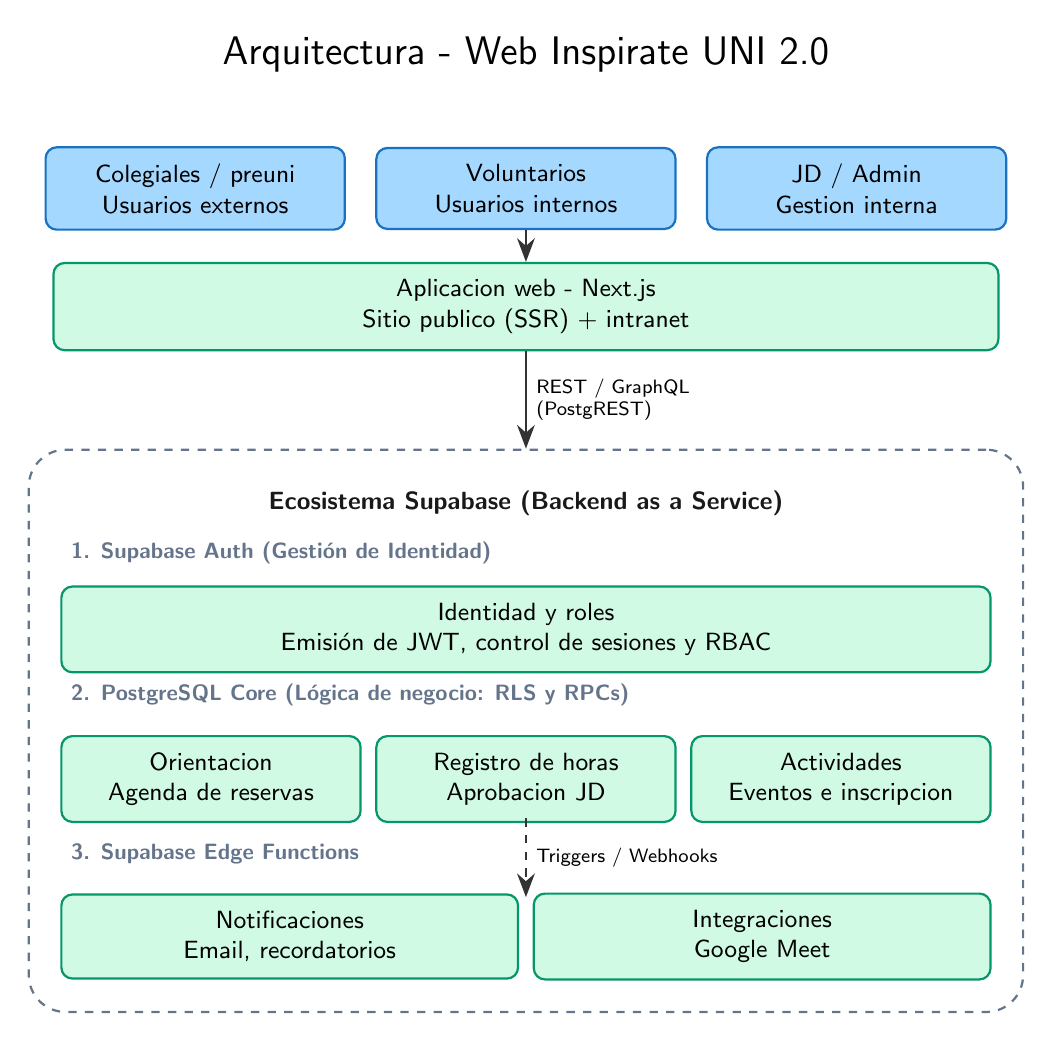
\begin{tikzpicture}

    % 1. Título
    \node[font=\Large] at (0, 3.5) {Arquitectura - Web Inspirate UNI 2.0};

    % 2. Fila Superior (Usuarios)
    \node[bluebox] (voluntarios) at (0, 1.8) {Voluntarios \\ Usuarios internos};
    \node[bluebox] (colegiales) at (-4.2, 1.8) {Colegiales / preuni \\ Usuarios externos};
    \node[bluebox] (admin) at (4.2, 1.8) {JD / Admin \\ Gestion interna};

    % 3. Aplicación Web
    \node[widegreenbox] (webapp) at (0, 0.3) {Aplicacion web - Next.js \\ Sitio publico (SSR) + intranet};

    % ==========================================
    % 4. ECOSISTEMA SUPABASE (Con yshift para bajar en conjunto)
    % ==========================================
    \begin{scope}[yshift=-1cm] % <--- Ajusta esta distancia según necesites
        
        % Título del ecosistema
        \node[font=\small\bfseries, text=black!90] (supabase_title) at (0, -1.2) {Ecosistema Supabase (Backend as a Service)};

        % -- Capa 1: Auth --
        \node[font=\footnotesize\bfseries, text=bordergray, anchor=south west] (auth_lbl) at (-5.9, -2.1) {1. Supabase Auth (Gestión de Identidad)};
        \node[greenbox, minimum width=11.8cm] (identidad) at (0, -2.8) {Identidad y roles \\ Emisión de JWT, control de sesiones y RBAC};

        % -- Capa 2: Database (Lógica Core) --
        \node[font=\footnotesize\bfseries, text=bordergray, anchor=south west] (db_lbl) at (-5.9, -3.9) {2. PostgreSQL Core (Lógica de negocio: RLS y RPCs)};
        \node[greenbox] (orientacion) at (-4.0, -4.7) {Orientacion \\ Agenda de reservas};
        \node[greenbox] (registro) at (0, -4.7) {Registro de horas \\ Aprobacion JD};
        \node[greenbox] (actividades) at (4.0, -4.7) {Actividades \\ Eventos e inscripcion};

        % -- Capa 3: Edge Functions (Lógica Asíncrona) --
        \node[font=\footnotesize\bfseries, text=bordergray, anchor=south west] (edge_lbl) at (-5.9, -5.9) {3. Supabase Edge Functions};
        \node[greenbox, minimum width=5.8cm] (notificaciones) at (-3.0, -6.7) {Notificaciones \\ Email, recordatorios};
        \node[greenbox, minimum width=5.8cm] (integraciones) at (3.0, -6.7) {Integraciones \\ Google Meet};

        % -- Caja Envolvente de Supabase --
        \node[draw=bordergray, thick, dashed, rounded corners=3ex, fit=(supabase_title) (auth_lbl) (identidad) (db_lbl) (orientacion) (registro) (actividades) (edge_lbl) (notificaciones) (integraciones), inner sep=0.4cm] (supabase_box) {};

        % Flujo interno Supabase
        \draw[mydashedarrow] (0, -5.2) -- (0, -6.2) node[midway, right, font=\scriptsize] {Triggers / Webhooks};

    \end{scope}

    % ==========================================
    % 5. Elementos Externos
    % ==========================================
    
    % Anotaciones Laterales (Costos ajustados al nuevo nivel de integraciones)
    % \node[font=\normalsize, text=textred, align=center] (costos) at (8.5, -7.7) {Buscar \\ costos de API};

    % ==========================================
    % Conexiones (Flechas)
    % ==========================================
    
    % Usuarios a Web App
    \draw[myarrow] (voluntarios.south) -- (webapp.north);
    
    % Web App a Supabase (PostgREST)
    \draw[myarrow] (webapp.south) -- (supabase_box.north) node[midway, right, font=\scriptsize, align=left] {REST / GraphQL \\ (PostgREST)};

    % Flecha de costos
    % \draw[myarrow, draw=textred, shorten >=2pt] (costos.west) -- (integraciones.east);

\end{tikzpicture}
\end{document}